% #############################################################################
% This is Chapter 4
% !TEX root = ../main.tex
% #############################################################################
% Change the Name of the Chapter i the following line
\fancychapter{Results}
%%%%%%%%%%%%%%%%%%%%%%%%%%%%%%%%%%%%%%%%%%%%%%%%%%%%%%%%%%%%%%%%%%%%%%%%
%                                                                      %
%     File: Thesis_Results.tex                                         %
%     Tex Master: Thesis.tex                                           %
%                                                                      %
%     Author: Francisco Azeredo                                        %
%     Last modified :  2 Jul 2015                                      %
%                                                                      %
%%%%%%%%%%%%%%%%%%%%%%%%%%%%%%%%%%%%%%%%%%%%%%%%%%%%%%%%%%%%%%%%%%%%%%%%
\label{chapter:Results}

\section{Information extraction and Structuring}
Some more complex multimodal models were tested in the beginning of the thesis for better information extraction.
\begin{itemize}
    \item \textbf{PrimaLayout}: Identifying and classifying regions such as text, tables, and images.
    \item \textbf{PubLayNet}: Segmenting documents into logical blocks.
    \item \textbf{Nougat}: An OCR engine that converts documents into markdown, preserving the hierarchy of chapters, sections, and subsections.
\end{itemize}
With testing, PrimaLayout, and PubLayNet promise good results with good training. This models unfortunately are not well trained yet, and need to be refined, as results were very unpredictable. Nougat was the engine used in case the pdf document doesn't have a text metadata.
\section{Weaviate Schema Example Study}
\label{sec:schema_example_study}

This section presents a concrete case study demonstrating how the Weaviate schema \ref{fig:weaviate_class} is used to enable semantic search that respects and leverages an existing organizational structure—rather than treating documents as isolated items. The organizational model follows the UML in Figure~\ref{fig:weaviate_class}, with classes \textit{Fluxo} (workflow), \textit{Etapa} (stage), \textit{Entidade} (entity), \textit{Pasta} (folder), \textit{Ficheiro} (file), and \textit{Metadados} (metadata). The goal is twofold:

\begin{itemize}
    \item \textbf{Structure-aware retrieval:} Queries can traverse relationships (e.g., workflow \(\rightarrow\) stages \(\rightarrow\) files) and return results grounded in that hierarchy.
    \item \textbf{Semantic augmentation:} Each class is vectorized so that hybrid search (lexical + semantic) can surface relevant objects even when exact keywords or IDs are unknown.
\end{itemize}

\subsection{Purpose and Scenario}
Consider a corporate repository where approvals and contracts are organized by \textit{Entidade} and \textit{Pasta}, while operational progress is tracked as \textit{Fluxo} with multiple \textit{Etapa}. A user asks for “documents about contract approvals.” A structure-aware semantic search should:
\begin{enumerate}
    \item Identify relevant \textit{Fluxo} and \textit{Etapa} that relate to approvals.
    \item Traverse to \textit{Ficheiro} objects within the appropriate \textit{Pasta}/\textit{Entidade}.
    \item Surface associated \textit{Metadados} to explain the result and enable filtering or summarization.
\end{enumerate}
This approach aligns with company retrieval needs, where organizational context (who owns what, where it lives, how it flows) is as important as the document content itself.

\subsection{Implementation Overview}
The implementation follows the UML with explicit collections for each class and cross-references mirroring relationships in the organizational structure. Each collection is created with properties and configured for vectorization and generative capabilities. Vectorization enables hybrid search across class instances; generative capabilities (via an Ollama model) support succinct, context-aware responses when appropriate.

\paragraph{Collections and Configuration}
Six collections are instantiated: \textit{Fluxo}, \textit{Etapa}, \textit{Entidade}, \textit{Pasta}, \textit{Ficheiro}, \textit{Metadados}. Each has a minimal textual property (e.g., \texttt{name}) and is configured with:
\begin{itemize}
    \item \textbf{Named vectorization} using a transformer encoder for semantic indexing.
    \item \textbf{Generative integration} (Ollama endpoint and model) to allow text generation grounded in retrieved context.
\end{itemize}

\paragraph{Experimental Setup}
For reproducibility, the schema uses a local Ollama endpoint (\url{http://host.docker.internal:11434}) with a sentence-transformer encoder (\texttt{sentence-transformers/all-MiniLM-L6-v2}) for embeddings and a lightweight generation model (\texttt{qwen2.5:latest}). In practice, named vectorization should reference the actual textual property (e.g., \texttt{source\_properties = \{\allowbreak "name"\}}) to ensure objects are properly embedded.

\paragraph{Cross-References}
References implement the hierarchy and traversal paths, for example:
\begin{itemize}
    \item \textit{Fluxo} \(\rightarrow\) \texttt{hasEtapas}, \texttt{belongsToFicheiros}, \texttt{belongsToPastas}.
    \item \textit{Etapa} \(\rightarrow\) \texttt{belongsToFluxo}, \texttt{hasFicheiros}.
    \item \textit{Entidade} \(\rightarrow\) \texttt{hasPastas}, \texttt{hasFicheiros}.
    \item \textit{Pasta} \(\rightarrow\) \texttt{hasEntidades}, \texttt{hasFluxos}, \texttt{hasFicheiros}.
    \item \textit{Ficheiro} \(\rightarrow\) \texttt{belongsToMetadados}, \texttt{hasEtapas}, \texttt{hasPastas}, \texttt{hasEntidades}.
    \item \textit{Metadados} \(\rightarrow\) \texttt{hasFicheiros}, \texttt{hasEtapas}, \texttt{hasPastas}, \texttt{hasEntidades}.
\end{itemize}
These links allow queries to traverse from workflows to stages to files, or from entities to folders to files and their associated metadata.

\paragraph{Sample Data and Tests}
To validate the schema, synthetic data is inserted across classes with consistent linking (e.g., multiple \textit{Entidade}, each with several \textit{Pasta}, each with multiple \textit{Ficheiro}, each with \textit{Metadados}; plus several \textit{Fluxo} with many \textit{Etapa}). The following test queries illustrate structure-aware and semantic retrieval:
\begin{itemize}
    \item \textbf{Fluxo \& Etapas:} Fetch \textit{Fluxo} objects with their \textit{Etapa} names to verify workflow-stage traversal.
    \item \textbf{Entidade hierarchy:} Fetch \textit{Entidade} with nested \textit{Pasta} \(\rightarrow\) \textit{Ficheiro} \(\rightarrow\) \textit{Metadados} to demonstrate hierarchical expansion.
    \item \textbf{Global semantic search:} Run a hybrid search across all collections for a free-text query (e.g., “contract approvals”) and sort results by semantic score, showing how relevant objects are surfaced even when users do not know the exact location or identifiers.
\end{itemize}

\subsection{Discussion and Takeaways}
This example shows that vector databases like Weaviate can support company semantic retrieval that is \emph{aware of organizational structure}. By aligning collections and references with the UML model and enriching each node with embeddings, the system enables:
\begin{itemize}
    \item \textbf{Explainable results:} Returned items include their position in the hierarchy (e.g., which entity/folder/workflow they belong to) and their linked metadata.
    \item \textbf{Flexible navigation:} Agents or users can start from any node (workflow, entity, file) and traverse to related items.
    \item \textbf{Robust querying:} Hybrid search compensates for inconsistent terminology while references maintain precise relationships.
\end{itemize}
In practice, this approach supports agentic retrieval flows that combine semantic ranking with graph-like traversal, improving precision and user trust when working within complex corporate repositories.


\section{Experiment with metadata extraction versus naive RAG}
\subsection{Dataset: LiHua-World}
The knowledge graph experiment uses the \emph{LiHua-World} corpus: a time-indexed set of short textual records organized into weekly folders (e.g., \path{week11/20260318_1510.txt}) and topical subfolders (e.g., \path{bakery_deliver/20260531.txt}). Each file contains concise, structured messages or notes about daily life events (meetings, deliveries, fitness plans, chats, travel, garden updates), often with implicit participants and locations. This format provides:
\begin{itemize}
    \item \textbf{Temporal signals:} timestamps encoded in filenames (YYYYMMDD\_HHMM) and dates inside texts, enabling ordering and interval reasoning.
    \item \textbf{Multi-actor context:} recurring names across files (e.g., Li Hua, Wolfgang, Jennifer) support relationship extraction.
    \item \textbf{Domain variety:} community garden, bakery deliveries, fitness training, entertainment, and travel, which stress-test entity and relation typing.
\end{itemize}

\subsection{Knowledge Graph Ingestion}
To construct a structure-aware index, the corpus is processed by the metadata extractor framework in section \ref{sec:metadata_extraction} that performs:\footnote{\label{footnote:entity_types} Entity types prioritized in this dataset reflect the questions asked most: \textbf{organization}, \textbf{person}, \textbf{location}, and \textbf{event}.}
\begin{itemize}
    \item \textbf{Entity extraction:} Named entities are identified and normalized into specified types \ref{footnote:entity_types}. Examples include people (Li Hua, Wolfgang), organizations (gym, bakery), locations (Central Park, basement), and events (promotion dinner, garden meeting).
    \item \textbf{Relation extraction:} Links between entities are inferred (e.g., \texttt{person -> event} attended, \texttt{organization -> event} announced, \texttt{person -> location} visited), with temporal anchors derived from filenames and text.
    \item \textbf{Object creation and cross-references:} Extracted entities become objects in the Weaviate schema; relations are stored as cross-references consistent with the UML-style design described earlier (Section~\ref{sec:schema_example_study}). Each object carries properties such as \texttt{name}, \texttt{timestamp}, \texttt{source\_path}, and optional \texttt{snippet} for provenance.
    \item \textbf{Vectorization:} Textual properties are embedded (e.g., \path{sentence-transformers/all-MiniLM-L6-v2}) to enable hybrid retrieval combining semantic scoring with graph traversal.
\end{itemize}

In this setup, answers were generated by our RAG system, which employed a sentence embedding model \textit{all-MiniLM-L6-v2} for retrieval embeddings and a local \gls{LLM}, \textit{Qwen2M}, for generation in the offline benchmark. 
Each generated answer was then compared against its gold reference using the evaluation metrics reported below. 
These experiments relied on local models to provide a cost-effective baseline; stronger results were observed with larger hosted models but were too expensive to run this benchmark.

The benchmark dataset consisted of 100 questions, categorized as follows:
\begin{itemize}
    \item \textbf{Single:} Direct factoid questions answerable from a single piece of evidence.
    \item \textbf{Multi:} Multi-hop or reasoning questions requiring synthesis of multiple facts, temporal or causal reasoning, or understanding relationships between events.
    \item \textbf{Null:} Questions for which there is insufficient information in the evidence to answer.
\end{itemize}

The experiment compares knowledge-graph–aware retrieval (Mini and Light) against a naive baseline.
Figure~\ref{fig:Lihua-World} presents the results across all metrics.
\begin{figure}[H]
    \centering
    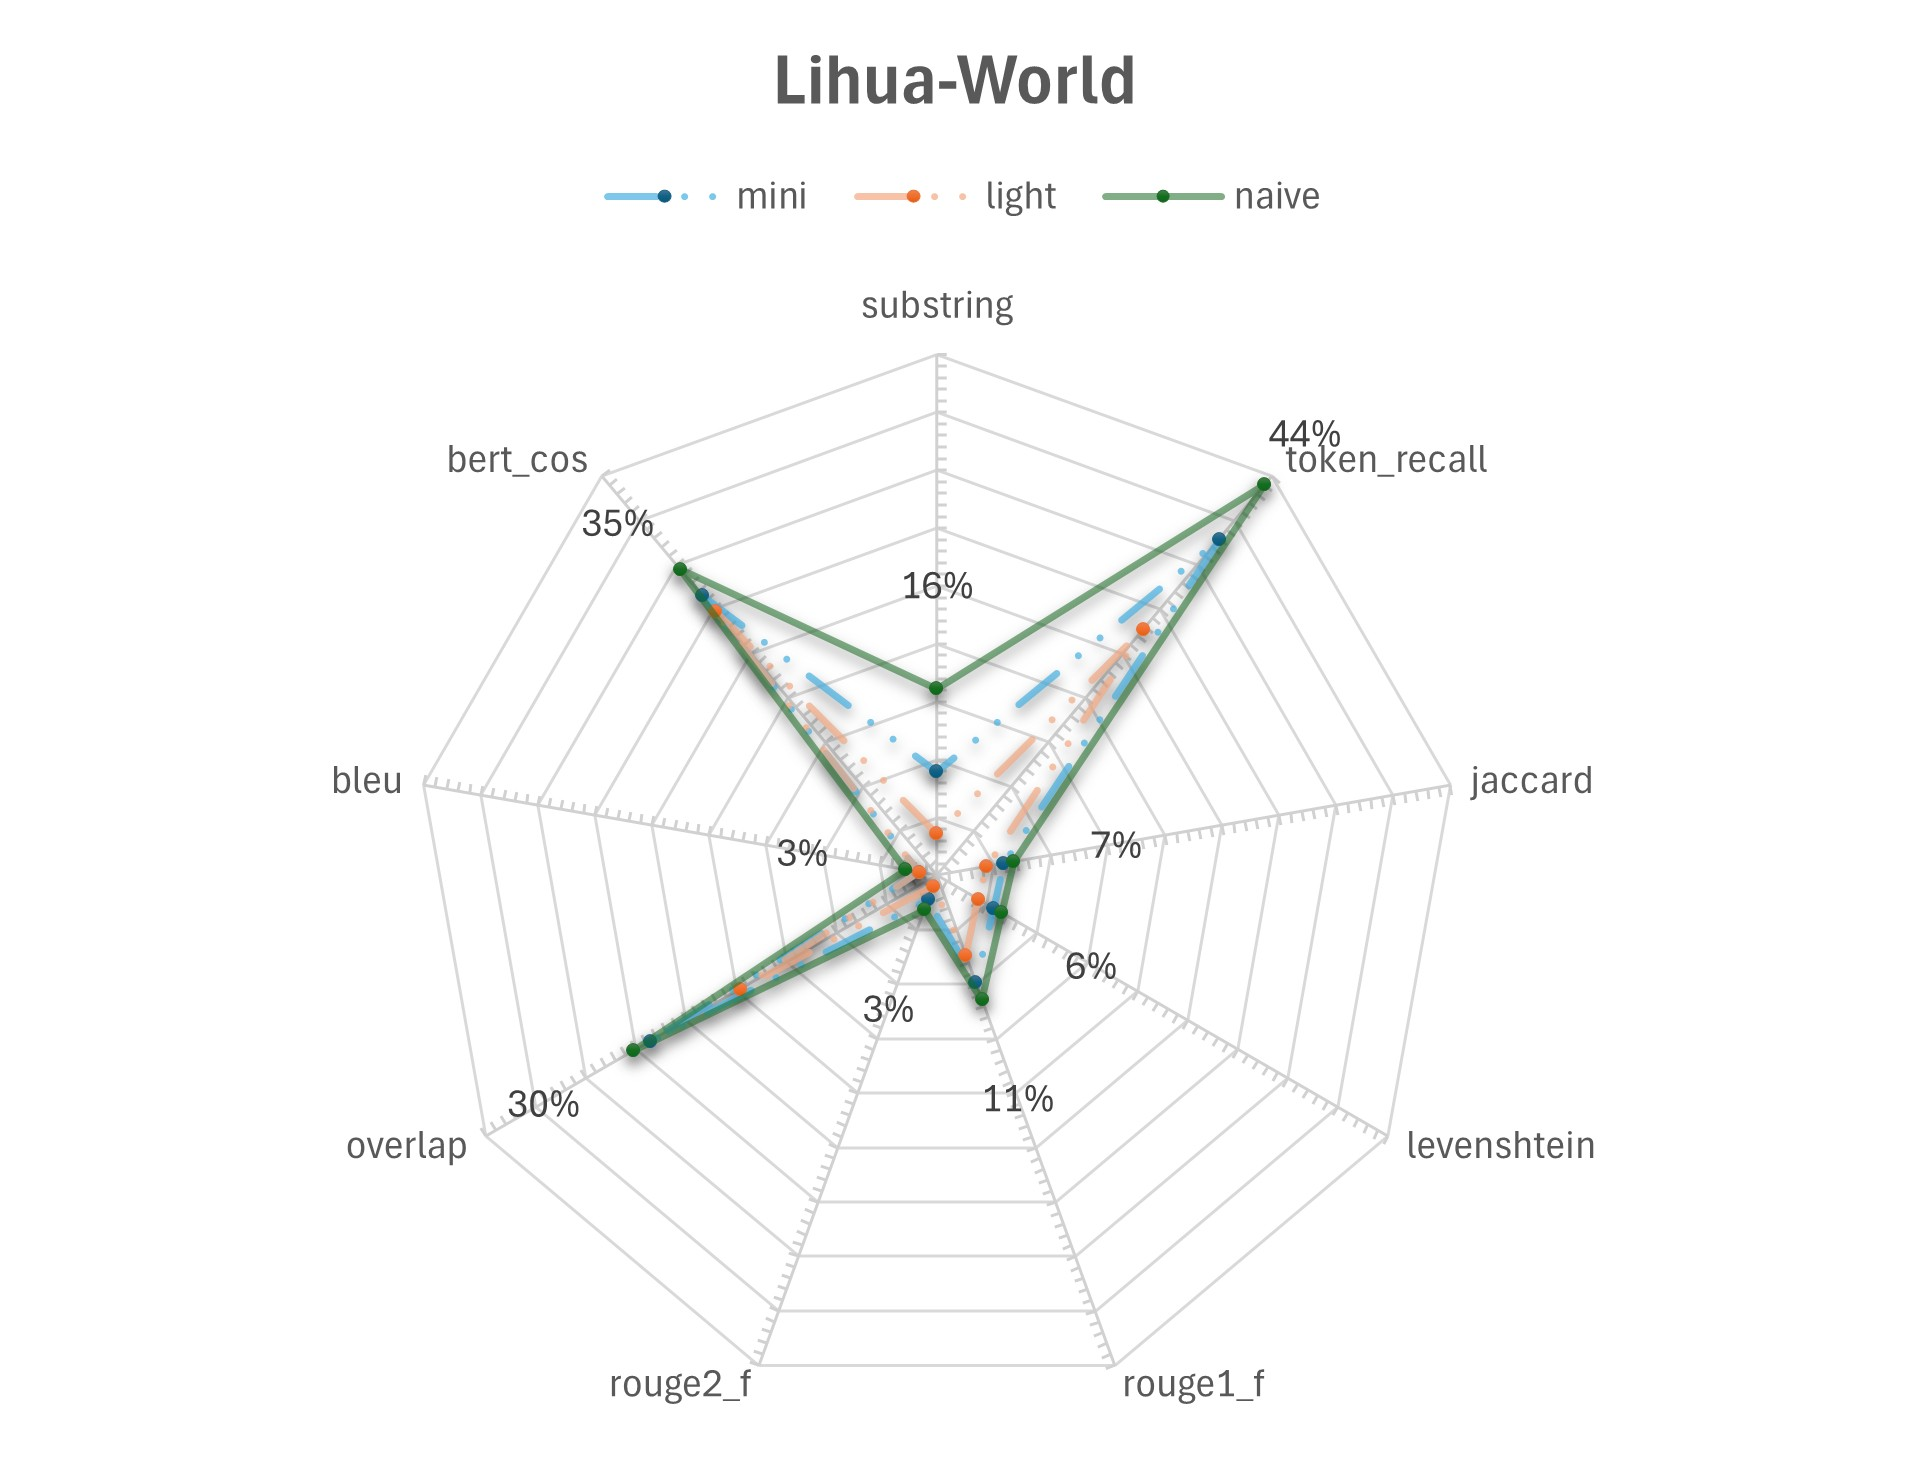
\includegraphics[width=1\linewidth]{Figures/Lihua-World.jpg}
    \caption{3 query types tested. With qwen2m as the llm and all-MiniLM-L6-v2 as embedding model}
    \label{fig:Lihua-World}
\end{figure}
Among the metrics, \textbf{Token Recall} achieved the highest score (44\%), and is the most relevant for this type of QA dataset.

\footnote{Note on metrics The full definitions and motivations for the evaluation metrics are provided in previous section \ref{sec:text-similarity-metrics}. Here we briefly reference the same set—lexical (Token Recall, Jaccard, Overlap), structural (Levenshtein, ROUGE, BLEU), and semantic (BERT cosine)—and focus on interpreting the results in this experiment.}

\subsection{Semantic Equivalence}
	\textbf{BERT cosine similarity} scored moderately (35\%). This is largely due to length imbalance between very short gold answers (sometimes a single token) and longer generated responses: sentence-level embeddings like \textit{all-MiniLM-L6-v2} capture global semantics, so single-token vs. full-sentence comparisons tend to yield low cosine values.

\subsection{Lexical Accuracy}
	\textbf{Token Recall} (44\%) confirms that correct essential tokens are often present in predictions. The \textbf{Overlap Coefficient} (30\%) is comparatively robust when lengths differ, since it does not penalize extra tokens. In contrast, \textbf{Jaccard} (7\%) suffers when generated answers are longer, inflating the union and suppressing the overlap proportion—even for partially correct outputs.

\subsection{Structural Similarity}
	\textbf{Levenshtein} (6\%) provides weak signal under large length differences. \textbf{ROUGE-1 F1} (11\%) and \textbf{ROUGE-2 F1} (3\%) partly mitigate this by balancing precision and recall over n-grams, but longer responses with irrelevant tokens reduce precision. ROUGE-2 is particularly low because short gold answers rarely contain bigrams. Finally, \textbf{BLEU} (3\%)—designed for machine translation—over-penalizes deviations and brevity mismatches in this setting, making it unsuitable here.

\subsection{Summary}
This experiment implemented an automated approach to forming a knowledge graph with semantic structure—mirroring a UML diagram for cross-references in Weaviate. The goal was to enable retrieval that leverages explicit entity relationships and organizational context, not just surface-level text.

However, results show that this automatic knowledge graph construction currently fails to reliably create a strong semantic structure for retrieval. In practice, direct embedding-based indexing (sentence transformers) remains faster and more effective for retrieval tasks, consistently outperforming the knowledge graph approach in this setup.

Profiling and structuring text with an LLM is also much more computationally expensive: each 200-token chunk is processed through a few-shot prompt (with many input tokens), up to three times, plus an additional pass for entity merging and summarization. This makes large-scale knowledge graph creation costly. While using a heavier LLM could improve the quality of the knowledge graph and its retrieval performance, the resource requirements and latency increase substantially.

In summary, while knowledge graphs offer richer structure and could become more competitive with stronger LLMs, current embedding models provide a more scalable and efficient solution for semantic retrieval. Future work may revisit knowledge graph approaches as LLM costs decrease and capabilities improve.

\section{Experiment: Naive vs.\ Agentic RAG with Company Information}
\label{sec:expNaiveVsAgenticRAG}
This experiment aims to evaluate the effectiveness of an agentic retrieval-augmented generation (RAG) approach compared to a naive RAG baseline in answering context-specific questions about company information. The goal is to determine whether an agent that plans and reasons over retrieved documents can provide more accurate and relevant answers than a straightforward retrieval and generation pipeline.

For this experiment, a synthetic company QA dataset was created in two automated stages:
\begin{enumerate}
        \item \textbf{Document Generation:} First, a set of 1000 realistic administrative documents was generated using a GPT-5 model. Each document was produced by prompting the model with a specific archival classification (from a public sector taxonomy), including its description, notes, and index terms, but instructing the model to never mention the class name in the content. The result is a diverse collection of plausible, well-structured company files, each corresponding to a different administrative or legal context. The total cost of generating these documents was around 5 dollars (around 10000 tokens per request).
        \item \textbf{QA Pair Generation:} \label{subsec:qa-generation} Next, for a random subset of these documents, a second generative model (also GPT-5) was used to create question-answer pairs. The model was prompted with the full content of each document and instructed to generate a specific, contextual question that could only be answered by reading that document, along with a precise answer based exclusively on its content. This ensures that each QA pair is tightly coupled to a single file and cannot be answered from general knowledge or other documents. The cost of generating 300 such QA pairs was around 0.85 dollars.
\end{enumerate}

This process yields the QA benchmark used to test developed RAG systems, where each question is answerable only by retrieving the correct company file and reasoning over its content. The dataset is well-suited for evaluating retrieval-augmented generation (RAG) systems, as it requires both accurate retrieval and grounded answer generation.

\subsection{Vector database setup}
The vector database used in this work is Weaviate. It is populated with 1000 synthetic company documents created earlier (see Section~\ref{sec:schema_example_study} and the dataset generation steps) and indexed using \texttt{sentence-transformers/all-MiniLM-L6-v2} embeddings. The schema is simple: a single class \textit{Ficheiro} (file) with properties \texttt{text} and \texttt{file\_path}. Each document is stored as one object, with \texttt{text} vectorized (named vector \texttt{text\_vector}) to support semantic search; \texttt{file\_path} stores the document source for grounding answers. This same index is used by both the naive and agentic systems in the subsequent experiments.

\subsection{Naive RAG and CoT Baseline}
\label{sec:naive-rag-and-cot-baseline}
The naive baseline retrieved top-ranked passages from Weaviate and generated an answer; the CoT variant used the same retrieval with a short step-by-step hint.
For each question in the QA dataset (generated in \ref{subsec:qa-generation}), the naive pipeline executes:
\begin{enumerate}
    \item Run a hybrid search in Weaviate (\(\alpha = 0.7\)) over \texttt{text\_vector} with the question to retrieve the top-$k$ objects containing \texttt{text} and \texttt{file\_path}.
    \item Generate a concise answer grounded in the retrieved content.
\end{enumerate}

At a high level, the naive pipeline performs a single retrieve-and-generate pass over hybrid search results in Portuguese. We iterated variants with \texttt{qwen2.5} to pick a cost-effective baseline, then re-ran the best with ChatGPT-5 to estimate upper-bound quality. See Algorithm~\ref{alg:naive-weaviate-hybrid} (Appendix~B) for details.
The results are presented in Figure~\ref{fig:weaviate_test}.
We use this as a control: it is simpler to implement and requires no large model for planning.
\begin{figure}
    \centering
    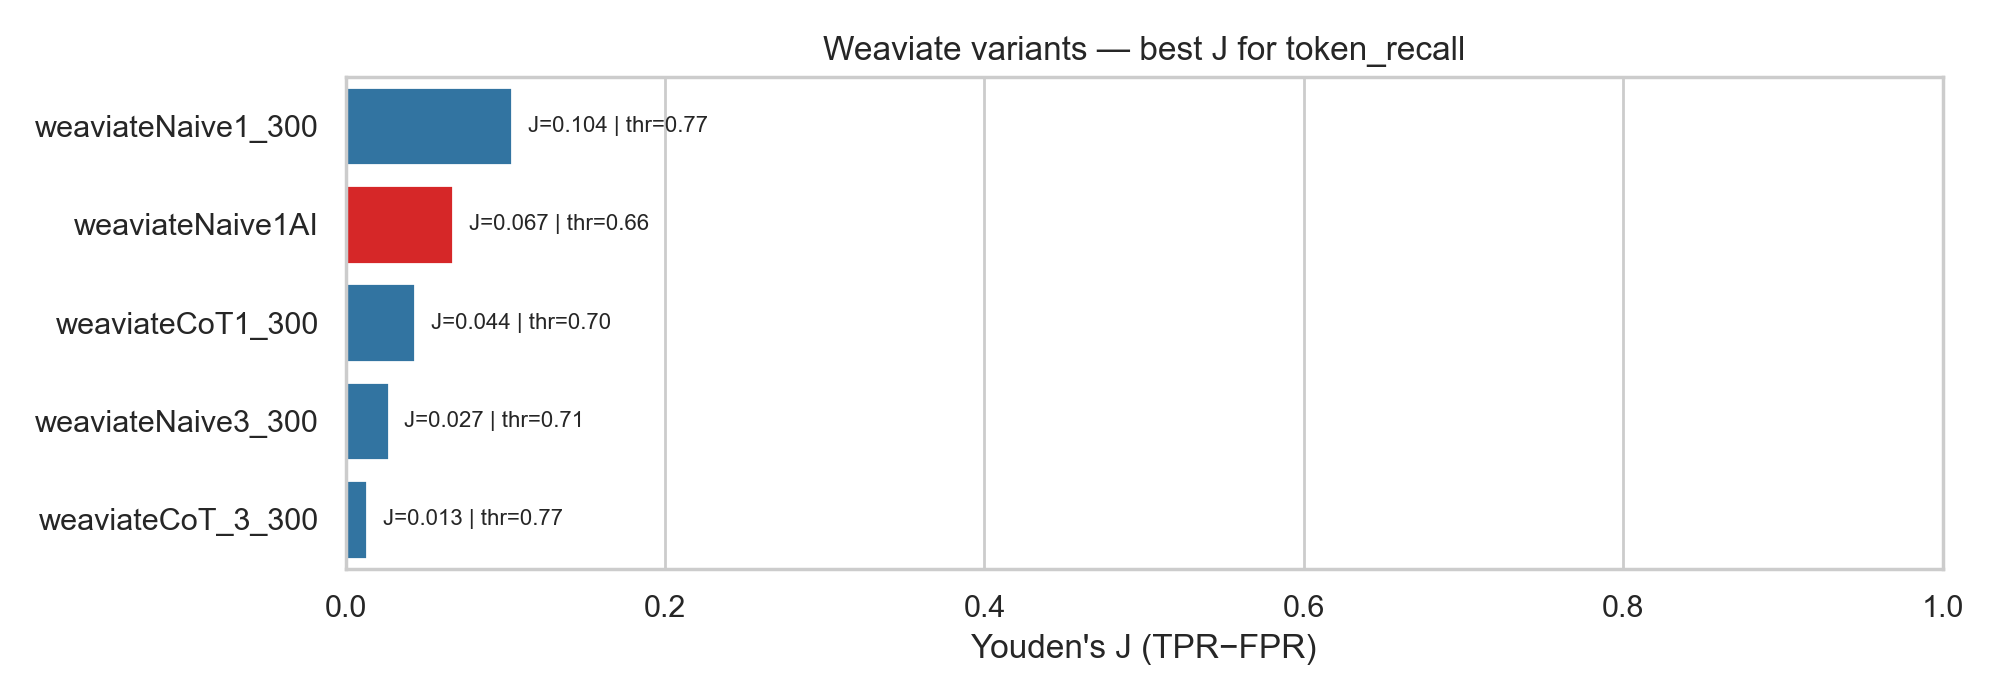
\includegraphics[width=1\linewidth]{Figures/10_weaviate_best_j_token_recall.png}
    \caption{Youden's J statistic for qualifying best naive rag variant. With qwen2.5m as the llm and all-MiniLM-L6-v2 as embedding model. And a chatgpt5 variant using best top-$k$ and prompt parameters.(k=4, prompt=naive)}
    \label{fig:weaviate_test}
\end{figure}
\subsection{Agentic Test}
\label{sec:agentic-test}

To set up the test, we developed a \textbf{ReAct} agent connected to a Weaviate vector database via \gls{MCP} developed in this thesis~\ref{sec:weaviate-mcp-server}.  Following initial trials with a local model (\texttt{qwen2.5m}) that exhibited frequent context drift, drifting from the question, leading to extractive outputs, reinforcing the need for a larger context window, we used \textbf{ChatGPT-5} for planning and generation, as a larger model is required to maintain multi-step reasoning within its context window.

\subsection{Agent Workflow}
For each question in the QA dataset (generated in \ref{subsec:qa-generation}), the agent follows a ReAct loop:
\begin{enumerate}
\item \textbf{Plan:} Sketch a brief strategy to find the answer.
\item \textbf{Retrieve:} Fetch the most relevant documents.
\item \textbf{Observe \& Reflect:} Inspect the evidence and, if needed, refine the plan and retrieval.
\item \textbf{Answer:} Produce a concise response grounded in the retrieved content.
\end{enumerate}

Across \textbf{300} questions, the agent sometimes required up to \textbf{20} LLM calls per question, with a total run cost of approximately \textbf{\$14}. Reasoning improves answer quality, but it significantly increases latency and cost compared to naive RAG.

\section{Quality Metric Evaluation}
\label{sec:metric-evaluation-quality}
To evaluate answer quality, we use the same metrics as in the previous experiment (Section~\ref{sec:expNaiveVsAgenticRAG}), but we analyse a step further by analyzing results with the theory that answers can only be correct if the source document is correctly retrieved. We analyse by seeing which threshold for a metric score to categorize a answer as correct, aligns with the source being correctly retrieved. The threshold is best when Youden's J statistic is maximized, which is defined as: The difference between true positive rate (TPR) and false positive rate (FPR).
\begin{figure}[H]
    \centering
    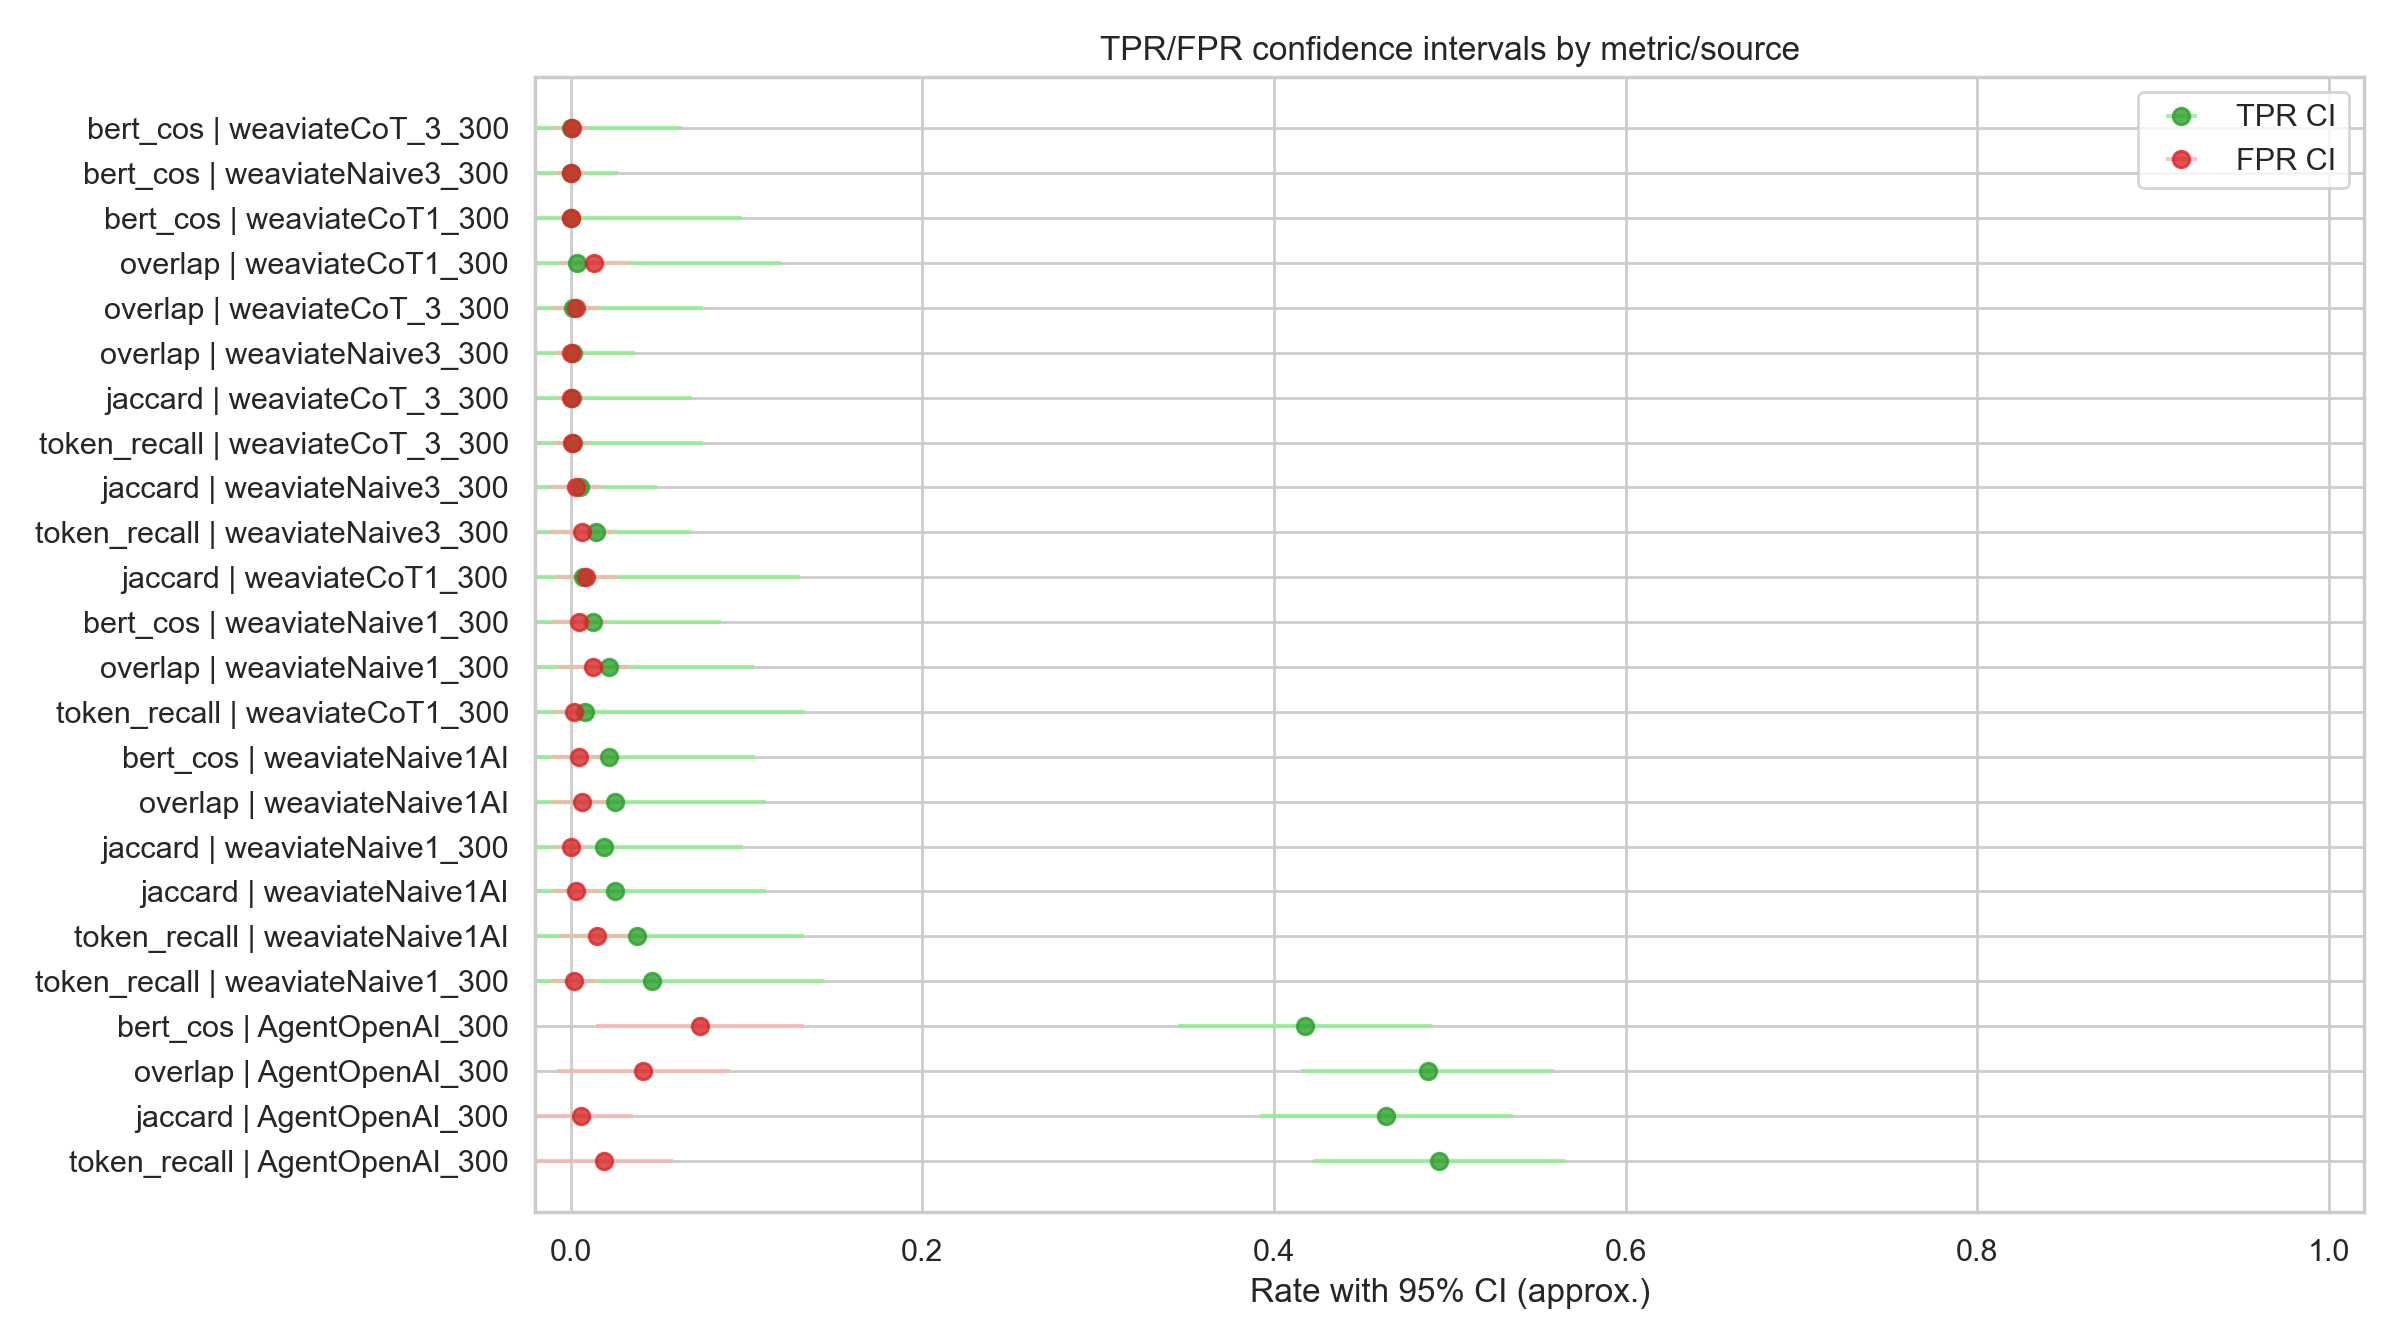
\includegraphics[width=1\linewidth]{Figures/06_tpr_fpr_confidence_intervals.png}
    \caption{confidence intervals for TPR and FPR per metric, for all source benchmark results, using the threshold that maximizes Youden's J statistic.}
    \label{fig:confidence-intervals}
\end{figure}

From the TPR and FPR confidence intervals figure \ref{fig:confidence-intervals}, we can observe that results benchmarked from the agentic RAG system have a much better quality than the naive RAG system, across all metrics. This indicates that the best benchmark to determine the best thresholds using Youden's J statistic, is the agentic RAG system. Part of the reason for Agentic RAG system having a better quality result is the fact that it is more balanced for missed retrievals, and true retrievals. As seen from the document retrieved percentage in table \ref{tab:doc-retrieved-by-source},
The Agentic RAG system retrieves more documents correctly than the naive RAG system. This is because the agentic RAG system can reason and plan, and therefore retrieve more relevant documents, while the naive RAG system only retrieves based on a single hybrid search.

\begin{table}[htbp]
    \centering
    \begin{tabular}{l c}
        \hline
        Source file & Correct document retrieved \\
        \hline
    AgentOpenAI\_300 & 60.4\% \\
    weaviateNaive3\_300 & 22.5\% \\
    weaviateNaive1\_300 & 13.8\% \\
    weaviateNaive1AI & 13.4\% \\
    weaviateCoT\_3\_300 & 9.4\% \\
    weaviateCoT1\_300 & 5.7\% \\
        \hline
    \end{tabular}
    \caption{Document retrieved percentage by source file}
    \label{tab:doc-retrieved-by-source}
\end{table}

\begin{table}[htbp]
  \centering
  \begin{tabular}{l c c c c}
    \hline
    Metric & Threshold & TPR & FPR & J \\
    \hline
    token\_recall & 0.67 & 56.7\% & 4.4\%  & 52.3\% \\
    jaccard       & 0.26 & 53.7\% & 2.0\%  & 51.7\% \\
    rouge1\_f     & 0.40 & 52.3\% & 2.7\%  & 49.7\% \\
    overlap       & 0.56 & 56.0\% & 7.7\%  & 48.3\% \\
    bleu          & 0.37 & 39.3\% & 1.3\%  & 37.9\% \\
    bert\_cos     & 0.71 & 49.0\% & 12.1\% & 36.9\% \\
    \hline
  \end{tabular}
    \caption{Best thresholds by metric (max True--False pass-rate difference) for File: AgentOpenAI\_300}
    \label{tab:agentopenai300-best-thresholds}
\end{table}

Table \ref{tab:agentopenai300-best-thresholds}

\subsection{Overall metric results}
From the last subsection, we conclude that the best metric thresholds (by Youden's J statistic) are obtained from the Agentic RAG system; we therefore use those thresholds to categorize answers as correct or incorrect across benchmarks. We also narrow down the analysis to the best naive RAG variant (weaviateNaive1\_300), using qwen2.5 and OpenAI models, and the agentic RAG system (AgentOpenAI\_300). The results are presented in figure \ref{fig:median-metric} and table \ref{tab:gain-loss-reference-median}. The median metric scores are also presented for reference.
\begin{figure}
    \centering
    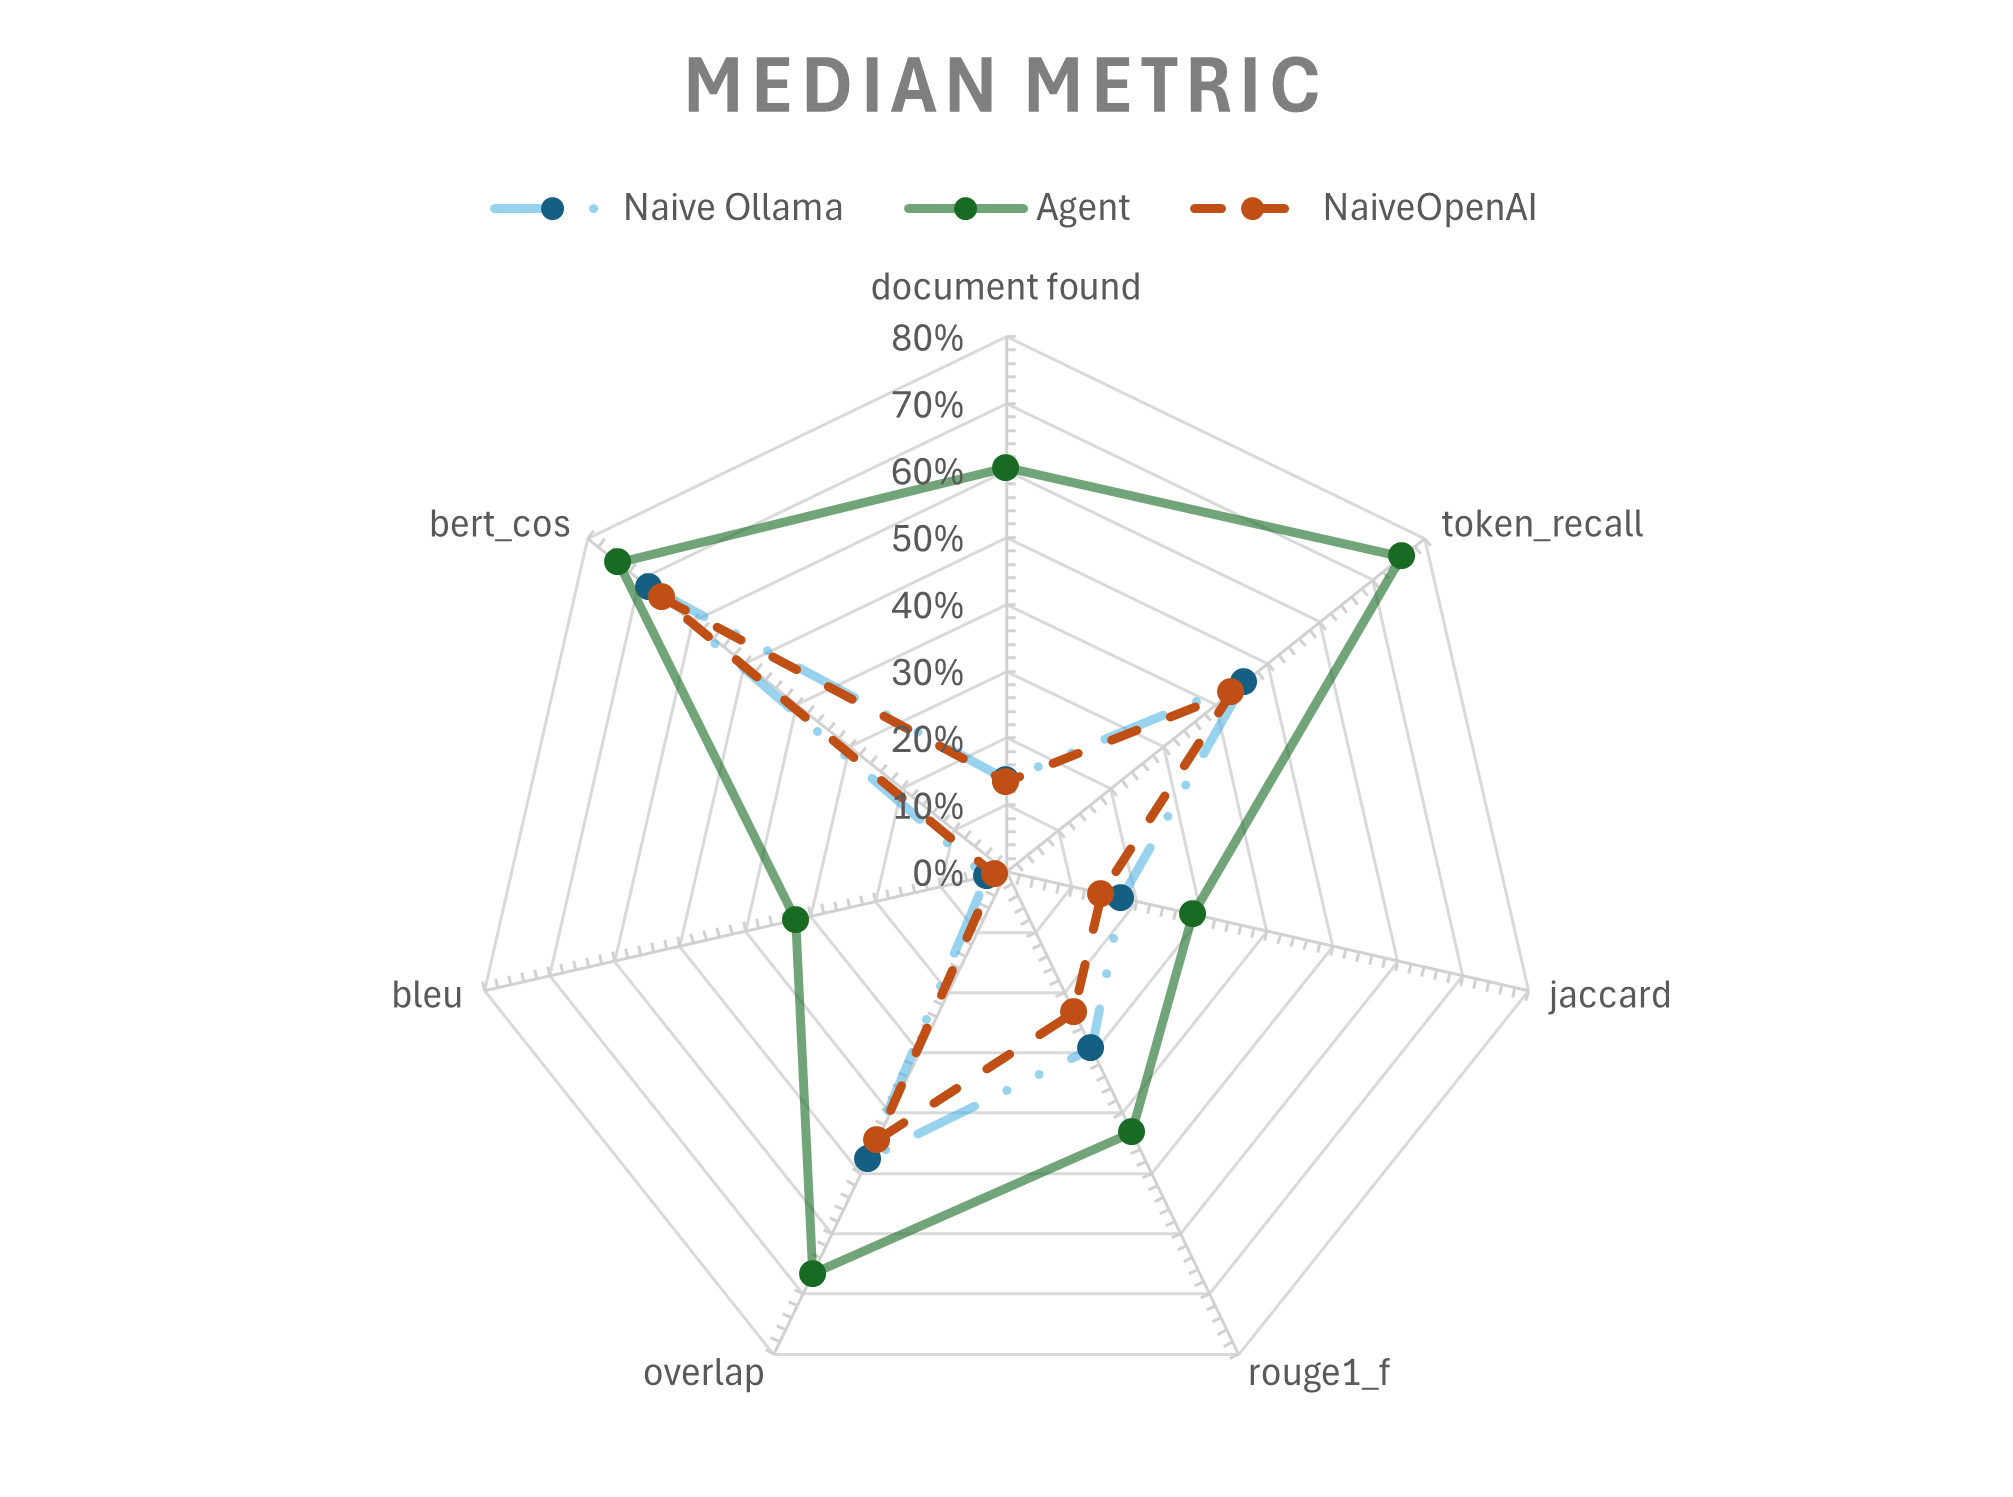
\includegraphics[width=0.75\linewidth]{Figures/Median Metric.png}
    \caption{Median Metric Scores}
    \label{fig:median-metric}
\end{figure}
According to Table~\ref{tab:agentopenai300-best-thresholds}, the metrics ranked by Youden's J are: \textbf{Token Recall}, \textbf{Jaccard}, \textbf{ROUGE-1 F1}, \textbf{Overlap}, \textbf{BLEU}, and \textbf{BERT cosine}. This ordering indicates which scores are most reliable for classifying answers as correct in this dataset. Token Recall tops the list because questions are specific and correctness hinges on including the right content words; surface fluency or paraphrase similarity is secondary. Conversely, BERT cosine, which emphasizes sentence-level semantic proximity, performs worst here because many gold answers are short and exactness is required. Jaccard also performs well by rewarding coverage of relevant tokens relative to the union, providing a useful proxy for answer completeness.

\begin{table}[htbp]
    \centering
    \begin{tabular}{l r r r  r r r}
        \hline
        benchmark &  token recall & jaccard & rouge1 & overlap & bleu & bert cosine \\
        \hline
        Agent OpenAI &  -15\% & 27\% & 12\% & -3\% & 8\% & -13\% \\
        Naive OpenAI &  -31\% & -1\% & -9\% & -16\% & 1\% & -38\% \\
        Naive Ollama &  -26\% & 5\% & -8\% & -9\% & -1\% & -30\% \\
        \hline
    \end{tabular}
    \caption{Numerical differences when using agentic reference thresholds (Youden-optimized)\ref{fig:Youden-metric} versus median-based \ref{fig:median-metric} thresholds for classifying answers (positive values indicate gains).}
    \label{tab:gain-loss-reference-median}
\end{table}

Applying the agentic reference thresholds yields clear gains for \textit{Agent OpenAI} on \textit{Jaccard} (+27\%), \textit{ROUGE-1} (+12\%), and \textit{BLEU} (+8\%), with a trade-off in \textit{Token Recall} (\textminus 15\%). \textit{BERT cosine} declines (\textminus 13\%) are expected given the stricter, token-accuracy oriented thresholding. The naive baselines exhibit broad declines—especially in \textit{Token Recall} and \textit{BERT cosine}—indicating that thresholds calibrated on higher-quality, better-retrieved agentic outputs do not transfer as well to weaker systems.
\begin{figure}
    \centering
    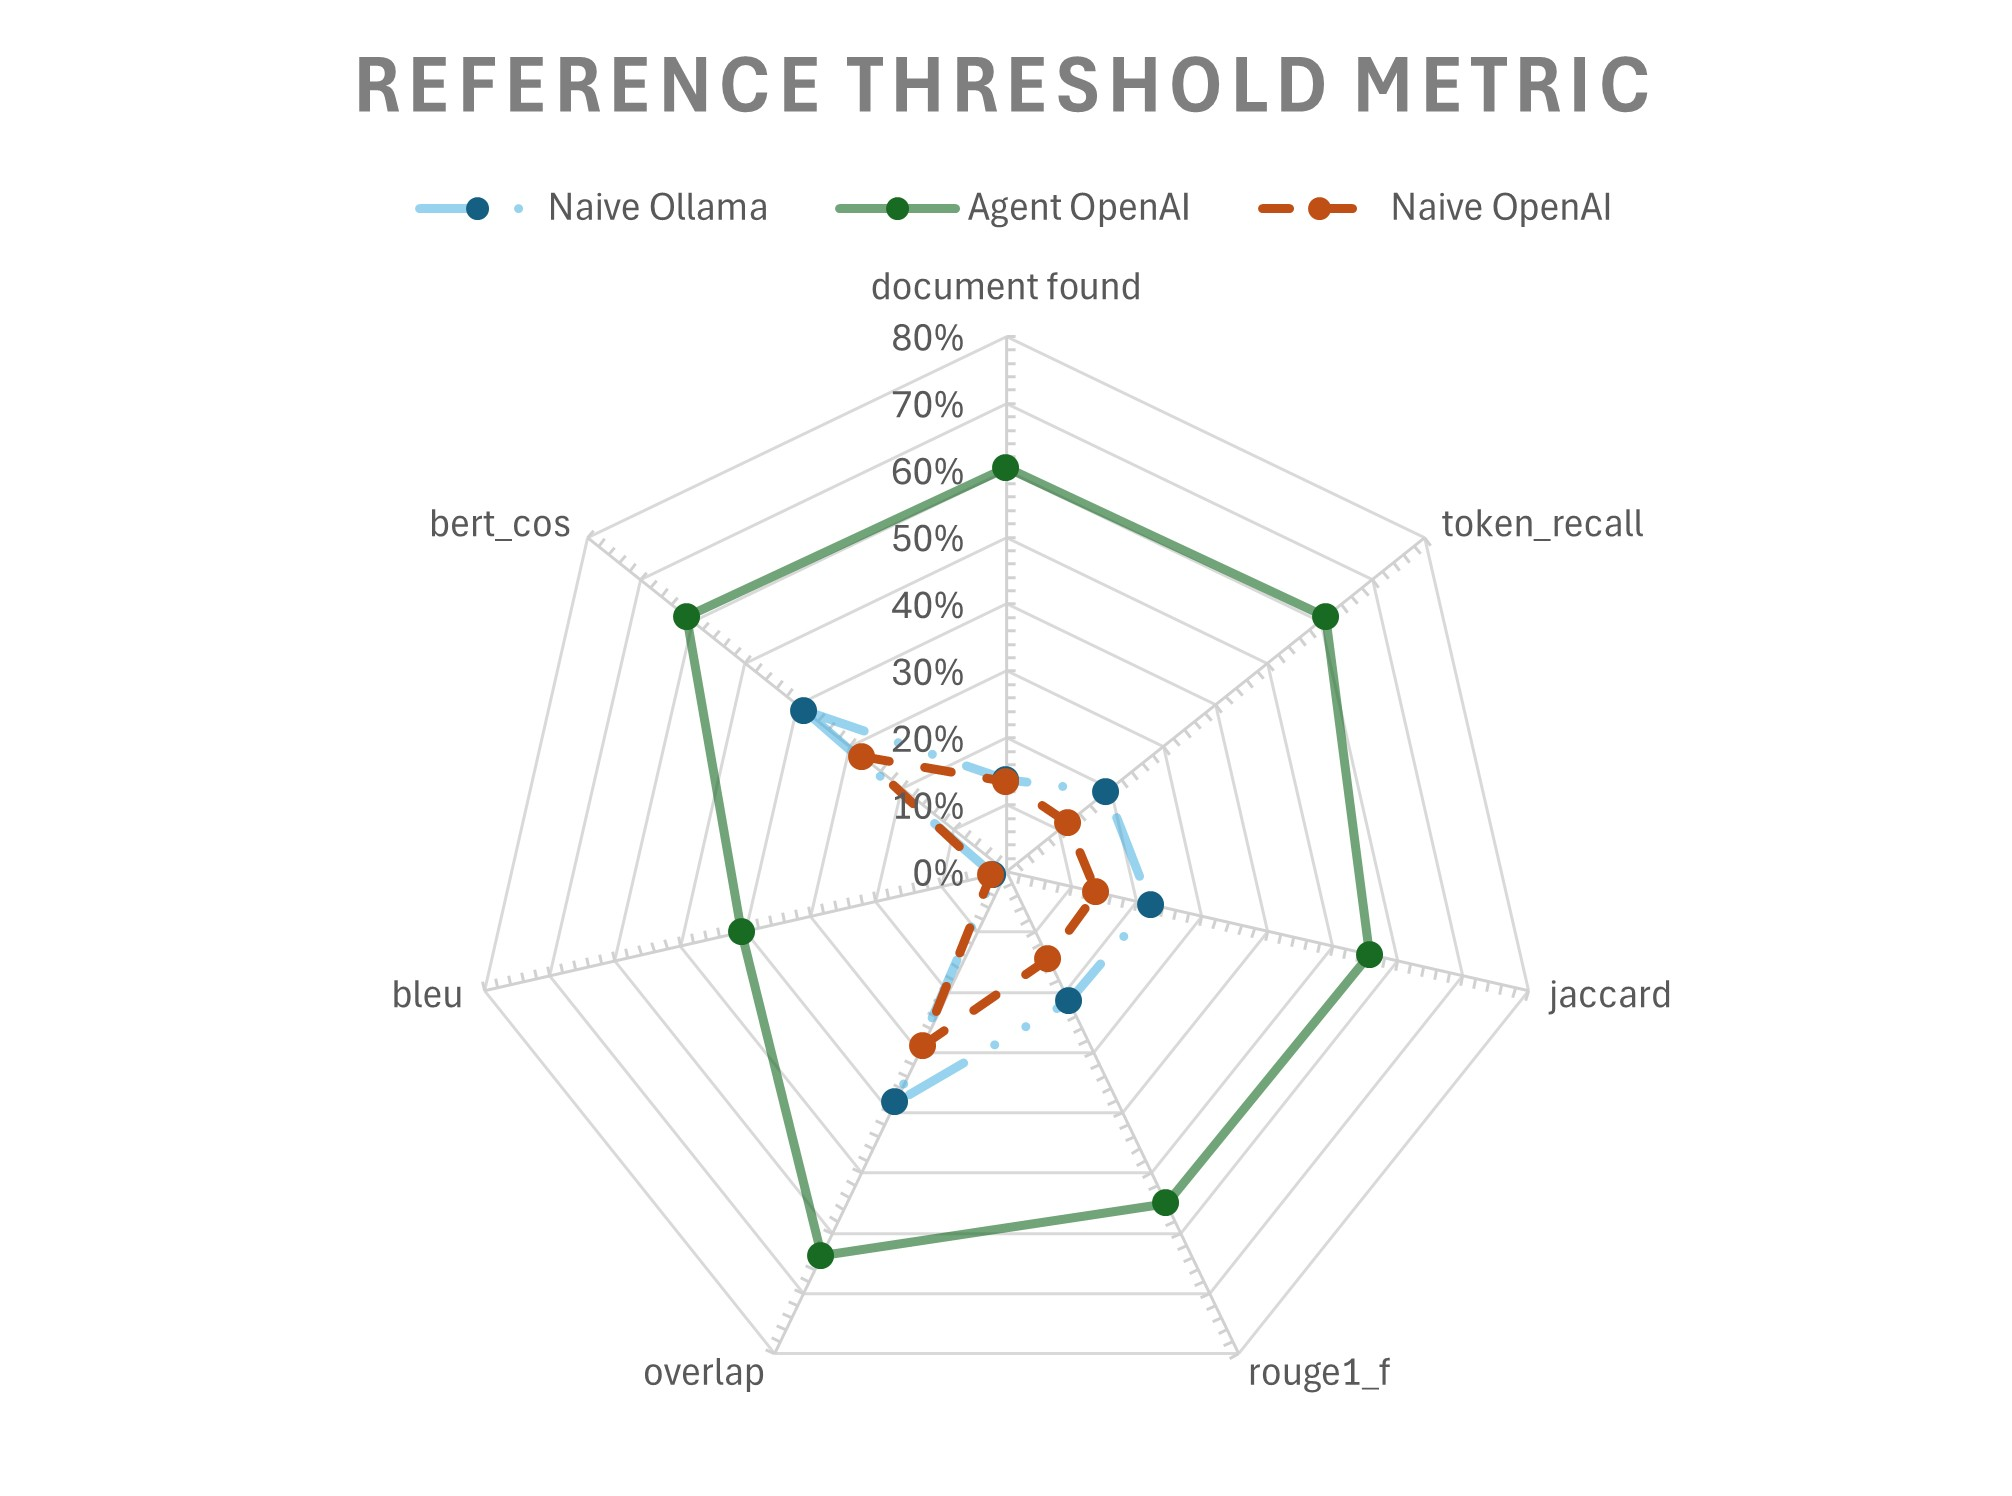
\includegraphics[width=0.75\linewidth]{Figures/Reference Threshold Metric.jpg}
    \caption{Agentic AI reference thresholds applied to all metrics of all important benchmarks}
    \label{fig:Youden-metric}
\end{figure}

Compared to the median-based thresholds, the agentic reference thresholds yield a more favorable profile for the \textit{Agent OpenAI} benchmark, boosting precision-oriented metrics (\textit{Jaccard}, \textit{ROUGE-1}, \textit{BLEU}) while sacrificing some recall (\textit{Token Recall}), but still remains a high score. This reflects the agent's ability to retrieve and synthesize relevant information more accurately, even if it occasionally omits less critical details. The naive baselines, however, do not benefit from this calibration, as their lower-quality outputs are less aligned with the stricter criteria derived from the agentic system.

\begin{table}[htbp]
    \centering
    \begin{tabular}{l r r r r r r}
        \hline
        benchmark & token\_recall & jaccard & rouge1\_f & overlap & bleu & bert cosine \\
        \hline
        Agent OpenAI & 61\% & 56\% & 55\% & 64\% & 41\% & 61\% \\
        Naive OpenAI & 12\% & 14\% & 14\% & 29\% & 2\% & 28\% \\
        Naive Ollama & 19\% & 22\% & 21\% & 38\% & 2\% & 39\% \\
        \hline
    \end{tabular}
    \caption{Share of answers passing Youden-optimized thresholds (Figure~\ref{fig:Youden-metric}); higher is better.}
    \label{tab:youden-metric-values}
\end{table}

Taken together with Figure~\ref{fig:Youden-metric}, these values show a pronounced separation between the agentic system and naive baselines under Youden-optimized criteria. The \textit{Agent OpenAI} workflow—plan, retrieve, observe/reflect, and answer—consistently classifies a much larger fraction of outputs as correct across metrics (e.g., 61\% Token Recall and 64\% Overlap), whereas naive pipelines lag substantially (e.g., Token Recall 12–19\%, Overlap 29–38\%). This evidences the benefit of iterative reasoning and refinement over a single-pass naive RAG. This is also coupled by the fact that agentic RAG retrieves more documents correctly than the naive RAG system, as seen in table \ref{tab:doc-retrieved-by-source}.





